\section{Generated convergence records and robustness figures}
\label{sec:supplement-convergence-robustness}

This section collects the generated records that accompany the executable
numerical specification in Supplementary Section~\ref{sec:spectral-numerics}.
The tables are regenerated from qualified artifacts and the registered
configuration; the figures read only the same artifacts and export the plotted
arrays to \path{data/source_data/supplementary}.  They are evidence for
discretization, phase, branch-tracking, differentiation, source-window, and
finite-anisotropy robustness within the declared ranges, not replacements for
the hypotheses of the perturbation and stationary-phase theorems.

\begin{table}[htbp]
  \centering
  \caption{Independent isotropic one-element and two-element convergence
  record.  The errors are relative to the high-precision Rayleigh--Lamb ZGV
  root; the residual and eigengap use the definitions in Supplementary
  Section~\ref{sec:spectral-numerics}.}
  \label{tab:supplement-convergence}
  \resizebox{\textwidth}{!}{% Generated from the deterministic auxiliary isotropic validation record.
\begin{tabular}{lrrrrrrr}
\hline
discretization & $p$ & elements & $|\delta\kappa_0|/\kappa_0$ & $|\delta\Omega_0|/\Omega_0$ & $|\delta a|/a$ & eigen residual & minimum eigengap \\
\hline
one element & 28 & 1 & 1.642797e-14 & 2.144017e-12 & 8.610456e-11 & 4.685472e-12 & 0.22289169 \\
two elements & 28 & 2 & 1.451459e-12 & 5.332013e-13 & 1.225559e-09 & 8.997835e-12 & 0.22289169 \\
\hline
\end{tabular}
}
\end{table}

\begin{table}[htbp]
  \centering
  \caption{Registered reference parameters, numerical tolerances, and the
  material record used only for the silicon stress test.  Dimensionless
  entries are read from the registered YAML configuration; the silicon constants
  retain their source identifier in the generated table.}
  \label{tab:supplement-parameters}
  \resizebox{0.86\textwidth}{!}{% Generated only from reference.yaml and silicon_stress_test metadata.
\begin{tabular}{lll}
\hline
parameter & value & provenance \\
\hline
$h$ & 1 & reference configuration \\
$\rho$ & 1 & reference configuration \\
$\lambda$ & 2 & reference configuration \\
$\mu$ & 1 & reference configuration \\
$\delta$ & 1 & reference configuration \\
$R/h$ & 0.5 & reference configuration \\
$\sigma/k_0$ & 0.15 & reference configuration \\
annulus fraction & 0.15 & reference configuration \\
eigen residual tolerance & 1.000000e-10 & reference configuration \\
isotropic match tolerance & 1.000000e-07 & reference configuration \\
curvature match tolerance & 1.000000e-04 & reference configuration \\
sensitivity match tolerance & 1.000000e-04 & reference configuration \\
phase error tolerance & 0.05 & reference configuration \\
$C_{11}$ (GPa) & 165.7 & doi:10.1107/S1600577514004962 \\
$C_{12}$ (GPa) & 63.9 & doi:10.1107/S1600577514004962 \\
$C_{44}$ (GPa) & 79.6 & doi:10.1107/S1600577514004962 \\
\hline
\end{tabular}
}
\end{table}

\begin{figure}[p]
  \centering
  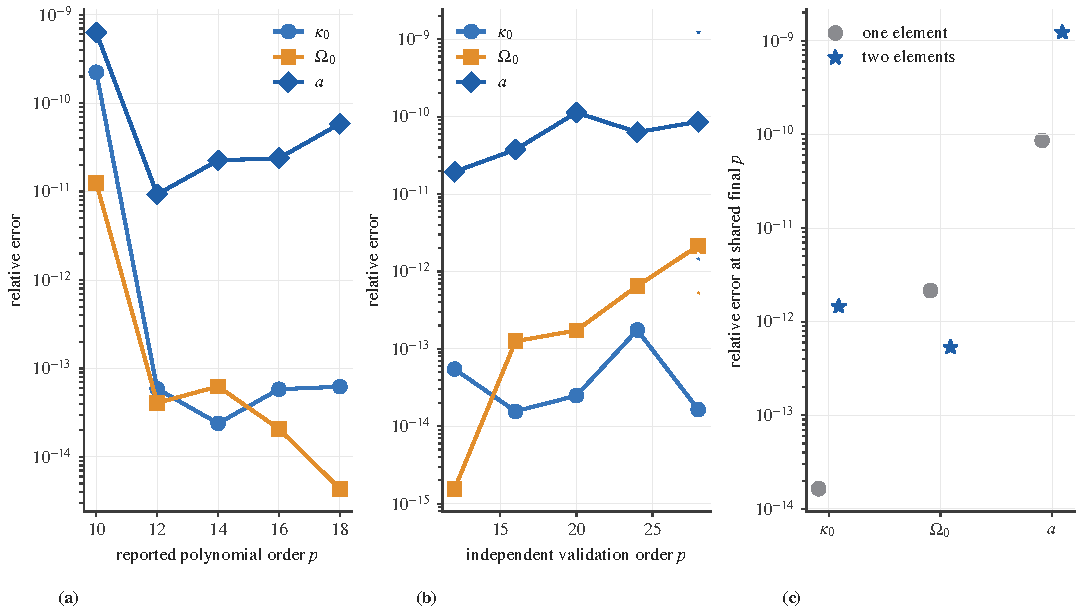
\includegraphics[width=\textwidth]{../figures/supplementary/figure_s01_polynomial_two_element.pdf}
  \caption{\SupplementaryFigureOneCaption}
  \label{fig:supplement-01}
\end{figure}

\begin{figure}[p]
  \centering
  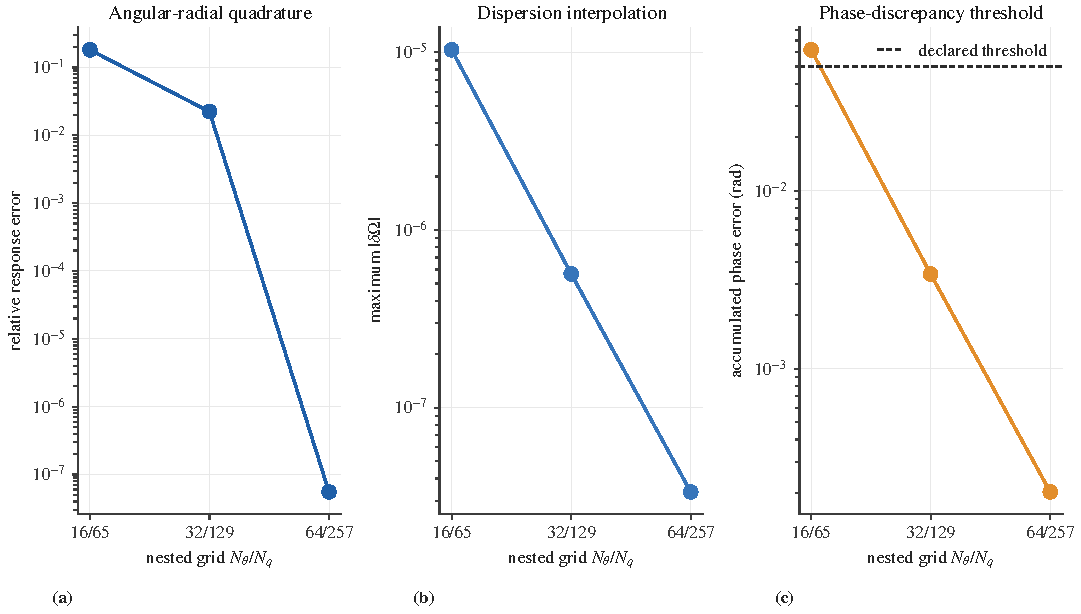
\includegraphics[width=\textwidth]{../figures/supplementary/figure_s02_quadrature_phase.pdf}
  \caption{\SupplementaryFigureTwoCaption}
  \label{fig:supplement-02}
\end{figure}

\begin{figure}[p]
  \centering
  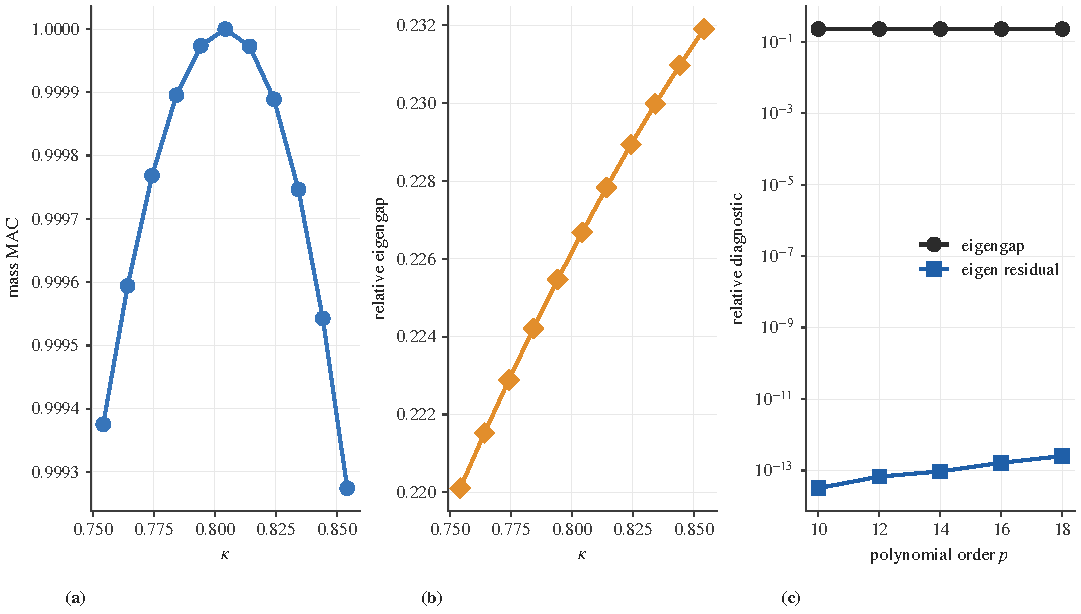
\includegraphics[width=\textwidth]{../figures/supplementary/figure_s03_mode_tracking.pdf}
  \caption{\SupplementaryFigureThreeCaption}
  \label{fig:supplement-03}
\end{figure}

\begin{figure}[p]
  \centering
  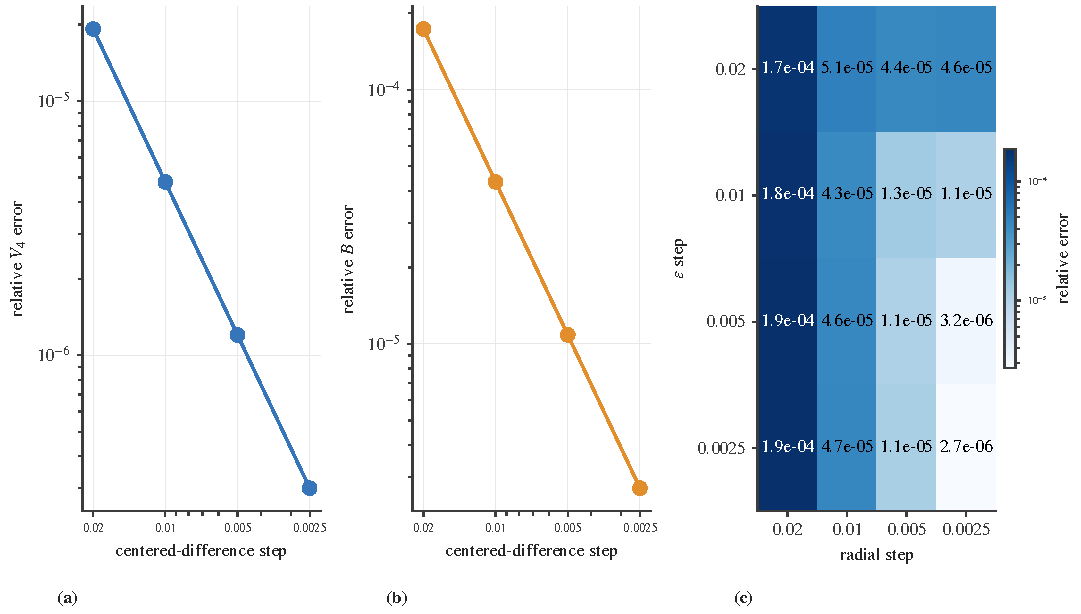
\includegraphics[width=\textwidth]{../figures/supplementary/figure_s04_fd_convergence.pdf}
  \caption{\SupplementaryFigureFourCaption}
  \label{fig:supplement-04}
\end{figure}

\begin{figure}[p]
  \centering
  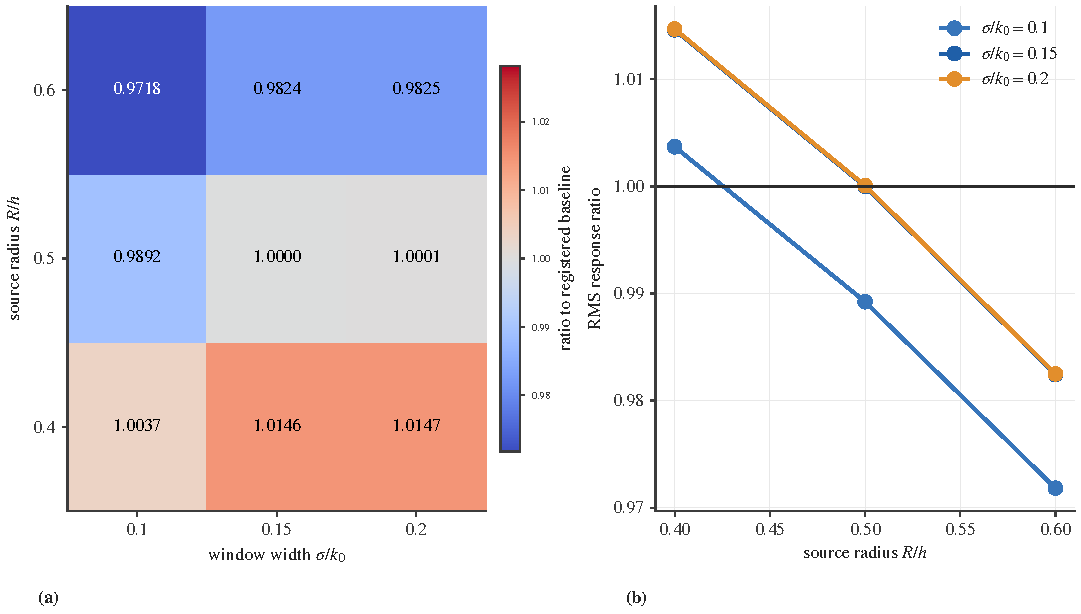
\includegraphics[width=\textwidth]{../figures/supplementary/figure_s05_source_window_sensitivity.pdf}
  \caption{\SupplementaryFigureFiveCaption}
  \label{fig:supplement-05}
\end{figure}

\begin{figure}[p]
  \centering
  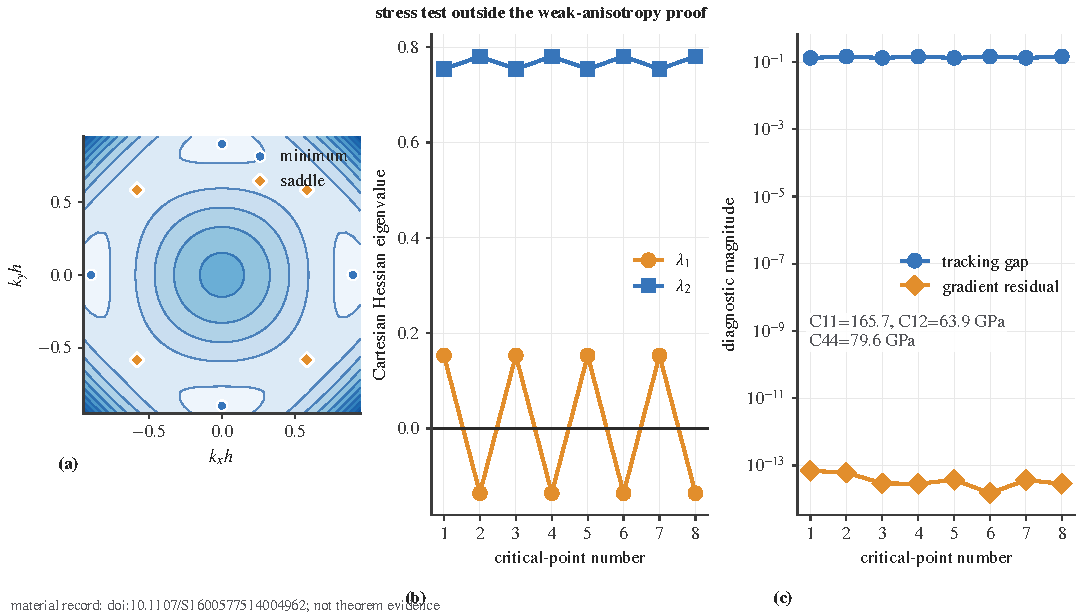
\includegraphics[width=\textwidth]{../figures/supplementary/figure_s06_silicon_stress_test.pdf}
  \caption{\SupplementaryFigureSixCaption}
  \label{fig:supplement-06}
\end{figure}

\clearpage
